\documentclass[../PiTest.tex]{subfiles}

\begin{document}

\section{Project definition}

    The project definition will be split in two sections, describing the server and on the client.

    \subsection{Server}
    The server application, from now on \pitest, is installed on the Operating System of the board and needs \nodejs\  to work.

    \subsubsection{Architecture diagram}
    The following is an high level diagram of the architecture of \pitest.
    
    \begin{figure}[!h]
        \centering
        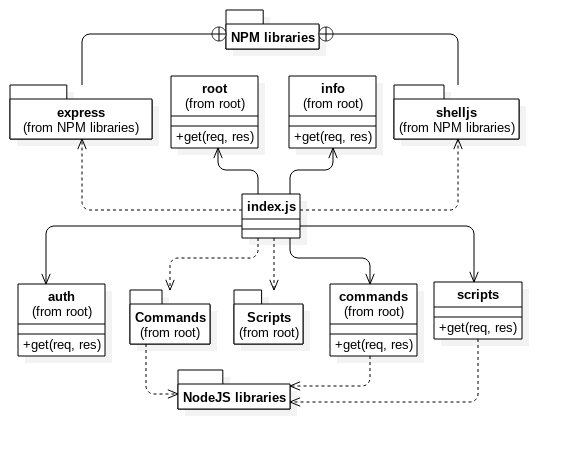
\includegraphics[width=\textwidth+1cm, height=10cm, keepaspectratio]{\detokenize{UML/png/Model__High level server diagram_1.png}}
        \caption{High level architectural diagram}
    \end{figure}

    \clearpage

    \subsubsection{Low level class diagram}

    \begin{figure}[!h]
        \centering
        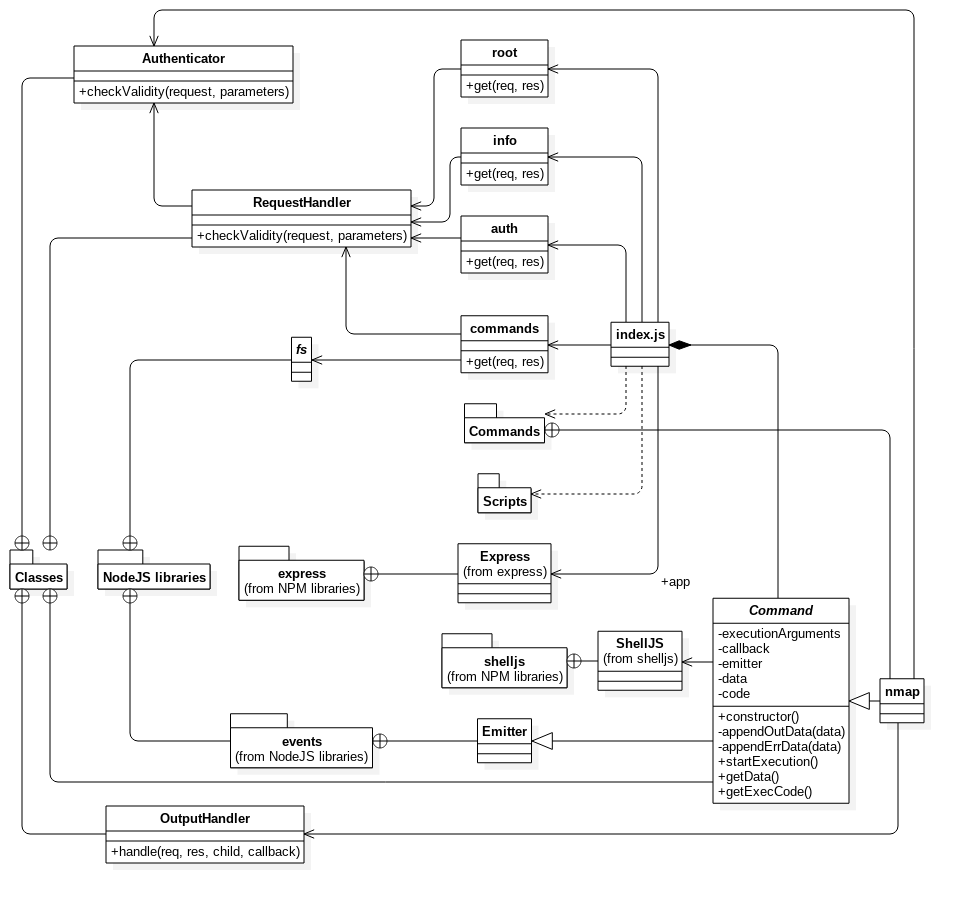
\includegraphics[width=\textwidth+1cm, keepaspectratio]{\detokenize{UML/png/Model__Low level server diagram_0.png}}
        \caption{Low level UML diagram of PiTest}
    \end{figure}

    \clearpage

    \subsubsection{Modules}

    \subparagraph{index.js}
    This is the main file of the application, it creates an Express app and loads all the routes of the web app.
    
    \subparagraph{root}
    Defines the behaviour of the root page (\texttt{/}), it is purpose is to respond with a custom welcome message.

    \subparagraph{info}
    Defines the behaviour of the root \texttt{/info}, it gives information about the server, as its name, version and author; it requires authentication using a valid token.

    \subparagraph{auth}
    Defines the behaviour of the root \texttt{/auth}, it is used to authenticate the user and requires a valid token.

    \subparagraph{scripts}
    Defines GTE behaviour of the root \texttt{/scripts}, it is used to list to the user the possible scripts and all their parameters; it requires authentication using a valid token.

    \subsubsection{Dependencies}
    Since the necessity of a solid code base from which extend the application, I have chosen to use some common libraries, from the standard \nodejs ones and from NPM modules.

    \subparagraph{fs}
    It is a \nodejs standard library which allows to read files on the file system.

    \subparagraph{events}
    It is a \nodejs standard library which allows to use the event system.

    \subparagraph{express}
    It is a \npm library which allows to generate a complete web server; it is used as a base for the \REST API. (\url{https://www.npmjs.com/package/express})

    \subparagraph{shelljs}
    It is a \npm library which allows to execute shell commands on the host in bot synchronous and asynchronous ways. It is used to call the host executables from the server.
    

    \subsubsection{Commands and scripts}
    To easily control the execution of commands and scripts I have chosen to create two respective wrapper classes, which contain all the information needed for the execution, have a simple interface to start the execution and retrieve the result with a callback. Also, every time there is an output, both on \texttt{STDERR} or \texttt{STDOUT} from the shell, an event, containing the relevant data, is created.

    \subsubsection{Virtualization for abstraction}
    Since not all applications can coexist on the same Operating System I have chosen to use \docker to separate and abstract the layer of control from the layer of execution. This way, it is possible to work with several distributions, in parallel, on the same system, and each one, possibly, with a different configuration.
    Every preconfigured command works on a \docker container, so the host is kept safe from possible vulnerabilities, while maintaining all its potential.

    \subsection{Client}
    The client side of the project is an Android application. I have chosen to use android as platform because it is the most common platform for mobile phones and ease access to all the libraries needed to do simple \REST calls. I have chosen this platform also because it is new to me, so I can learn something new with this project.

    \subsubsection{Dependencies}
    \subparagraph{Apache HTTP client}
    Used to manage the \REST calls and retrieve the information from the server.

    \subsubsection{Interface}
    The interface of the client will allow the user to setup the connection to the server with an authentication test. Next, if the connection is correct, the main menu, allowing the user to execute an arbitrary command, execute a preconfigured command or execute a preconfigured script.
    If the user choose to execute an arbitrary command, he will be prompted with a text box to enter it and an execute button. After the execution is completed, a text view will be populated with the text result.
    If the user choose to execute a preconfigured script or command, he will be prompted with a list of possible choices, each one with a simple description.
    Selecting an entry will start the execution; after which completion a text view will be populated with the result. Some preconfigured commands and scripts can have a custom view, to better show the results achieved.

    \subsubsection{REST calls}
    Every communication ongoing between the client and the server is through a \REST API. This way the client can manage multiple asynchronous commands in parallel and maintain an high level of security, as every call needs to be authenticated by a token. I have chosen to use \REST as it is more battery efficient than his common alternative, using a websocket, since it does not keep the connection open, sending ping-pong packets. Also, \REST is very simple to port on other platforms, allowing further expansion of the project.

    \subsubsection{Output customization}
    The use of a GUI allow to show the output of the server with a simple interface, which can be less intimidating than a shell for a non experienced user. An example would be a \textit{airodump-ng} scan, better presented with a list of items, with each own description.

\end{document}
